\documentclass[a4paper,twoside, openright, 12pt, leqno]{article}

% Upload template for articles


\usepackage{lipsum}  
\usepackage{graphicx}
\usepackage{amsmath, amssymb, bm}
\usepackage{booktabs}
\usepackage{ArticleTemp}

                  % Number theorems
%\usepackage{multirow}                    % Multiple rows in tables
%\usepackage{placeins}                    % Use \FloatBarrier to put figures and tables in current section

% TABLES: Alignment columns    
%\usepackage{array}
%\newcolumntype{L}[1]{>{\raggedright\let\newline\\\arraybackslash\hspace{0pt}}m{#1}}
%\newcolumntype{C}[1]{>{\centering\let\newline\\\arraybackslash\hspace{0pt}}m{#1}}
%\newcolumntype{R}[1]{>{\raggedleft\let\newline\\\arraybackslash\hspace{0pt}}m{#1}}


% Customize headers
\pagestyle{fancy}
\fancyhf{}
\fancyhead[RO,LE]{\small\thepage}
\fancyhead[LO]{\small \nouppercase{FertMort project}}
\fancyhead[RE]{\small \nouppercase{Camarda \& Aburto [Draft]}}
\fancyfoot[L,R,C]{}
\renewcommand{\headrulewidth}{0.4pt}

% Proposition with no numbering
% \newtheorem{proposition}{Proposition}
%\newtheorem*{proposition}{Proposition}
 
% Begin document
\begin{document}

% Remove header from the first page
\thispagestyle{empty}

% Affilations as footnotes with symmbols
% \renewcommand{\thefootnote}{\fnsymbol{footnote}}
\renewcommand{\thefootnote}{\alph{footnote}}

% Hyperlinks in title in black (Except E-Mail address)
\hypersetup{allcolors = black, footnotecolor = black, urlcolor = blue}

\begin{center}
    
    \vspace*{.4cm}
    \LARGE{Forecasting vital rates from demographic summary measures}    
    \vspace{.4cm}
   
    %\hypersetup{footnotecolor=black}
           
   \vspace{1cm}
    \large Giancarlo Camarda\footnote{Institut national d'\'etudes d\'emographiques.  E-Mail: \href{mailto:carlo-giovanni.camarda@ined.fr}{carlo-giovanni.camarda@ined.fr}} and Jos\'e Manuel Aburto\footnote{Interdisciplinary Centre on Population Dynamis University of Southern Denmark \& Max Planck Institute for Demographic Research  E-Mail: \href{mailto:jmaburto@sdu.dk}{jmaburto@sdu.dk}\label{SDU}} 
    %and Fernando Colchero\textsuperscript{\ref{MaxO}}\fnsep\footnote{Department of Mathematics and Computer Science, University of Southern Denmark, Odense, Denmark.}
    
    \vspace{1cm}
    \large\today
    \vspace{1cm}
    
\end{center}

% In text use numbers for footnotes
\renewcommand{\thefootnote}{\arabic{footnote}}
\setcounter{footnote}{0}

% All hyperlinks in blue in text
\hypersetup{allcolors = blue, footnotecolor = blue}

\section*{Abstract}


% Line interpsace
\linespread{1.5}\normalsize
\clearpage

\section{Introduction}
Future levels of mortality and fertility can be predicted by modelling and extrapolating rates over age and time, or by forecasting summary measures of each phenomena and then convert to age-specific rates. For example, in developed countries, the linear increase in life expectancy over some periods has made it easier to fit trends over time of this summary indicator than fitting more complex models based on age-specific dynamics of mortality \citep{White200259}. Therefore, several methods have been proposed to forecast life expectancy. For instance, \citet{torri2012forecasting} forecast life expectancy for a given country assuming a tendency towards a predicted best practice life expectancy. \citet{pascariu2018double} proposed incorporating the analysis of the gap between female and male life expectancy to more accurately predict the overall level of mortality in a country. Similarly, \citet{Raftery2013} forecast life expectancy for several countries using a Bayesian hierarchical model for females, and then model the sex gap to estimate male life expectancy \citep{raftery2014joint}. Subsequently, the overall level of mortality given by life expectancy is converted to a age-specific profile \citep{vsevvcikova2016age}. This latter method has been adopted by the United Nations. However, life expectancy, as an average, conceals the variation in the age-at-death distribution \citep{van2018case}. While the sources of variance in lifespans, or the health inequalities it reflects, are not fully understood, they however are a key problem for policy as well for modelling and forecasting mortality \citep{tuljapurkar2011variance}. Recently, \citet{bohk2017lifespan} proposed to incorporate the variation in ages at death as an additional indicator to evaluate mortality forecast. This variation is often called lifespan variation or lifespan inequality and refers to how similar ages at death are in a population.
They found that some methods struggle to account for trends in lifespan variation, which results in a mismatch between life expectancy and lifespan variation. In most countries, life expectancy and lifespan variation are often negatively correlated \citep{Smits2009,Vaupel2011,colchero2016emergence, alvarez2019latin, gonzaga2018compression}, however in some countries this association is less strong when looking at first differences over time. For example, in Central and Eastern European countries and in some Latin American countries life expectancy and lifespan variation moved independently from each other in periods when life expectancy improvements slowed-down \citep{Aburto2018Eastern,aburto2019upsurge,garcia2019impact}. This pattern is also more frequent in recent decades in low mortality countries \citep{aburtoDynamics2019}. Therefore, incorporating the dynamics of both life expectancy and lifespan variation to obtain an age-specific mortality profile that matches both is a step forward on more accurately predicting future longevity and the mechanisms underpinning new patterns in mortality.

In fertility forecasting, the challenge of accurately predicting levels and age-specific fertility dynamics rises from the complex association between structural changes (e.g. trajectory of total fertility) and changing age patterns (tempo) \citep{Booth2006}.  In general, forecasts of completed fertility aim to predict the number of children by women in reproductive age.  There are two big strands in fertility forecasting. (1) Cohort fertility, which is informative on what a cohort of women experience. Regarding (1), \citet{bohk2018forecast} compared the performance of 20 major methods, including parametric curve fitting methods, extrapolation, Bayesian approaches and context-specific methods, aimed at completing lifetime fertility of women that have not yet reached their last reproductive age. The authors found that more complex methods do not necessarily outperform simpler methods. The second strand is period fertility, which summarizes fertility within a period and central for our paper \citep{bohk2018forecast}. As in mortality forecasting, there is the case that total fertility or mean age at childbearing are forecasted \citep{miller1986bivariate}, but then there is the challenge of getting age-specific fertility rates consistent with those forecasts. \citet{lee1993modeling} modelled age-specific fertility rates over time imposing lower and upper bounds and an ultimate level of fertility to address the issues rising from structural change. Later on, \citet{lee1994stochastic} used this method with a different ultimate level of fertility and without bounds. Similarly, another approach to avoid the problem of structural change is setting a target total fertility (e.g. the average expectation of a group of experts) and then again face the problem of deriving age-specific dynamics \citep{lutz1996world}. To overcome this challenge, \citet{thompson1989multivariate} forecasted the total fertility rate, the mean age at childbearing, and the standard deviation of the age at childbearing using the gamma distribution and then estimated age-specific fertility rates from these parameters. Others, rely on probabilistic projections of the total fertility rate (TFR). For example, \citet{alkema2011probabilistic} developed a methodology to forecast TFR for all countries using a Bayesian projection model. To get the age-specific fertility patterns, the age patterns of fertility are projected based on past national trends combined with a trend leading towards a global model age patter of fertility \citep{vsevvcikova2016age, UN2017}. The final projection is a weighted average of two preliminary, and somehow arbitrary, projection scenarios. However, important information in other summary measures such as variance of childbearing age is often ignored \citep{hruschka2016does}. Our method pertains to this last method to derive age-specific fertility rates in the case that an aggregated summary measure such as TFR or mean age at childbearing is forecasted along with the standard deviation of the age at childbearing or other measure of variation. 

Here we propose a model to obtain future mortality and fertility age-patterns that comply with two projected summary measures (e.g. life expectancy and lifespan variation, or TFR and standard deviation of age at childbearing). Unlike comparable approaches, we assume only smoothness of future vital rates which is achieved by a two-dimensional $P$-spline approach as in \citet{currie2004smoothing}. Since summary measures are commonly nonlinear functions of the estimated penalized coefficients, Lagrangian multipliers cannot be directly implemented. We hence opted for a Sequential Quadratic Programming (SQP) procedure \citep{nocedal2006sequential} to perform the associated constrained nonlinear optimization. We formalize the model and illustrate our approach with mortality of Italian females, based on future life expectancy predicted by United Nations World Population Prospects \citep{UN2017} and future trends of lifespan disparity obtained by time-series analysis. We apply, additionally, our model to Spanish fertility constrained to total fertility rates, mean and variance of age at childbearing derived by time-series analysis.

\section{Methodology}

\subsection{Data}
We use data on deaths and population counts from the World Population Prospects for Italian females from 1960-1965 to the latest period 2010-2015 available. To test our model we use the projected life expectancy to 2050 and estimated future values for lifespan disparity using standard time series techniques with the projected death and population counts \citep{UN2017}. We also apply our model to fertility. For this we use data from the World Population Prospects for the total fertility rate (TFR) \citep{UN2017}, and age-specific births and population from the Human Fertility Database for Spanish females \cite{HFD}.

\subsection{Model on Italian mortality data}


For ease of presentation, we formulate the model on mortality data. Suppose that we have deaths, and exposures to risk, arranged in two matrices, 
$\bm{Y} = (y_{ij})$ and $\bm{E} = (e_{ij})$, both with dimension $m \times n_{1}$.  Rows and columns are classified by age at death, $\bm{a}, \,m \times 1$, and year of death, $\bm{t}_{1}, \,n_{1} \times 1$, respectively.  
We assume that the number of deaths $y_{ij}$ at age $i$ in year $j$ is Poisson distributed with mean $\mu_{ij} \,e_{ij}$, where $\mu_{ij}$ is the force of mortality. 
The aim of our model is to reconstruct trends in $\mu_{ij}$ for  $n_{2}$ future years, $\bm{y}_{2}, n_{2} \times 1$.

We arrange data as a column vector, that is, $\bm{y} = \verb"vec"(\bm{Y})$ and $\bm{e} = \verb"vec"(\bm{E})$ and we model our Poisson death counts as follows: $\ln(E(\bm{y})) = \ln(\bm{e})+ \bm{\eta} = \ln(\bm{e})+ \bm{B}\,\bm{\alpha}\, , $ where $\bm{B}$ is the regression matrix over the two dimensions: $\bm{B} = \bm{I}_{n_{1}} \otimes \bm{B}_{a}$, with $\bm{B}_{a} \in \mathbb{R}^{m \times k_{a}}$. Over time, we employ an identity matrix of dimension $n_{1}$ because we will incorporate a constraint for each year. Over age, $\bm{B}_{a}$ includes a specialized coefficient for dealing with mortality at age 0. In order to forecast, data and bases are augmented as follows:
%
\begin{equation}\label{eq:AugData}
\breve{\bm{E}} = [\bm{E} : \bm{E}_{2}]\, , \qquad 
\breve{\bm{Y}} = [\bm{Y} : \bm{Y}_{2}]\, , \qquad
\breve{\bm{B}} = \bm{I}_{n_{1}+n_{2}} \otimes \bm{B}_{a}
\, ,
\end{equation}
%
where $\bm{E}_{2}$ and $\bm{Y}_{2}$ are filled with arbitrary future values. If we define a weight matrix $\bm{V} = \mathrm{diag}(\verb"vec"(\bm{1}_{m\times n_{1}}:\bm{0}_{m\times n_{2}}))\,$, the coefficients vector $\bm{\alpha}$
can be estimated by a penalised version of the iteratively reweighted least squares algorithm: 
%
\begin{equation}\label{eq:penIRWLSfor}
(\breve{\bm{B}}^{T} \bm{V} \tilde{\bm{W}} \breve{\bm{B}} + \bm{P}) \tilde{\bm{\alpha}} =
\breve{\bm{B}}^{T}\bm{V} \tilde{\bm{W}}\tilde{\bm{z}} \, ,
\end{equation} 	
%
where a difference penalty $\bm{P}$ enforces smoothness behaviour of mortality both over age and time. 
%Outcomes from this approach in terms of life expectancy and $e^{\dagger}$ are depicted with a dashed line in Figure~\ref{fig:CamardaMort} (top panels), and departures from the UN and time-series projected values are evident. 

\subsubsection{Life expectancy and lifespan disparity}

Demographers and actuaries often summarize mortality age-patterns with life expectancy at  birth ($e^0$) (Figure~\ref{fig:CamardaMort}a). Life expectancy at birth is the average years a newborn is expected to live given the current mortality rates. Life expectancy is a nonlinear function of the coefficients vector $\bm{\alpha}$. In matrix notation, life expectancy at birth is defined as
%
\begin{equation}\label{eq:e0}
e^{0} (\bm{\alpha}_{j}) =  \bm{1}_{m}^{T} \, \exp[ \bm{C} \, \bm{\mu}_{j}]  + 0.5, 
\end{equation}
%
where $\bm{\mu}_{j} = \exp(\bm{B}_{a}\bm{\alpha}_{j})$ denotes mortality for a year $j$ and associated $k_{a}$ coefficients $\bm{\alpha}_{j}$, and $\bm{C}$ is a $(m \times m)$ lower triangular matrix filled only with -1.

Time-trends of this summary measure are often regular and well-understood. Forecasting a single time-series is therefore relatively easy. In recent years, measures of lifespan disparity have been incorporated to summarize population health alongside life expectancy \citep{van2018case}. Lifespan variation can be measured with multiple indicators \citep{vanRaalte2013}. These indicators are highly correlated when they measure variation over the full age range, i.e. starting from birth \citep{colchero2016emergence}. Here we measure lifespan variation with two indicators: 1) years of life lost ($e^\dagger$) and 2) the Gini coefficient of survival lifetimes. Results for the Gini coefficient are reported in the Supplementary Material.

Years of life lost, denoted with $e^\dagger$, is defined as the average remaining life expectancy when death occurs, see Figure~\ref{fig:CamardaMort}b \citep{Vaupel2003,Vaupel2011}. It is an indicator of absolute variation in lifespans. For example, when death is highly variable, some people will die well before their expected age at death, contributing many lost years to life disparity. When survival is highly concentrated around older ages, the difference between the age at death and the expected remaining years decreases, and life disparity decreases. In matrix notation is expressed as 
%
\begin{equation}\label{eq:ed}
e^{\dagger} (\bm{\alpha}_{j}) =  - \exp[ \bm{C} \, \bm{\mu}_{j}]^{T} \, \bm{C} \bm{\mu}_{j},
\end{equation} 
%
which is equivalent to the notation in lifetable functions $e^\dagger = -\int_0^\infty\, \ell(x)\,\ln{\ell(x)}\, dx
$ where $\ell(x)$ is the survival function. As life expectancy, $e^\dagger$ is a nonlinear function of the coefficients vector $\bm{\alpha}$. Therefore, constrained nonlinear optimization is necessary and a SQP approach is implemented. [I need to explain more about SQP]


 
Denote with $\bm{N}^{0}$ and $\bm{N}^{\dagger}$ the $(k_{a}n_{2} \times n_{2})$ matrices with block-diagonal structures containing derivatives of~\eqref{eq:e0} and \eqref{eq:ed} with respect to $\bm{\alpha}_{j}$ for $j=n_{1}+1, \ldots n_{1}+n_{2}$:
\begin{eqnarray}\label{eq:Der}
\frac{\partial e^{0} (\bm{\alpha}_{j})}{\partial \bm{\alpha}_{j}} &=& \bm{1}_{m}^{T} \verb"diag"[\exp(\bm{C}\bm{\mu}_{j})] \,	\bm{C} \,\verb"diag"(\bm{\mu}_{j}) \bm{B}_{a}\\
\frac{\partial e^{\dagger} (\bm{\alpha}_{j})}{\partial \bm{\alpha}_{j}} &=& - \bm{B}_{a}^{T} \left\{ \bm{C}^{T}[\bm{C}\bm{\mu}_{j} \circ \exp(\bm{C}\bm{\mu}_{j})] \circ \bm{\mu}_{j} \right\} + \nonumber\\
&& - \bm{B}_{a}^{T} \left\{ [\bm{C}^{T} \exp(\bm{C}\bm{\mu}_{j})] \circ \bm{\mu}_{j} \right\} \nonumber\, ,
\end{eqnarray}
where $\circ$ represents element-wise multiplication. Target life expectancy and lifespan disparity for future years are given by $n_{2}$-vectors $\bm{e}^{0}_{\mathrm{T}}$ and $\bm{e}^{\dagger}_{\mathrm{T}}$.

Solution of the associated system of equations at the step $\nu + 1$ is given by
\begin{equation}\label{eq:SQLalg}
\left[ \begin{array}{l}
\bm{\alpha}_{\nu+1}\\
\bm{\omega}_{\nu+1}
\end{array}\right] = 
\left[ \begin{array}{lllll}
\bm{L}_{\nu}  &:& \bm{H}^{0}_{\nu} &:& \bm{H}^{\dagger}_{\nu}\\
\bm{H}_{\nu}^{0 T}  &:& \bm{0}_{n_{2} \times n_{2}}&:&\bm{0}_{n_{2} \times n_{2}}\\
\bm{H}_{\nu}^{\dagger T} &:& \bm{0}_{n_{2} \times n_{2}} &:& \bm{0}_{n_{2} \times n_{2}}
\end{array}\right]^{-1}
\left[ \begin{array}{c}
\bm{r}_{\nu} - \bm{L}_{\nu}\bm{\alpha}_{\nu}\\
\bm{e}^{0}_{\mathrm{T}} - \bm{e}^{0} (\bm{\alpha}_{\nu})\\
\bm{e}^{\dagger}_{\mathrm{T}} - \bm{e}^{\dagger} (\bm{\alpha}_{\nu})\\
\end{array}\right] \, ,
\end{equation}
where $\bm{L}$ and $\bm{r}$ are left- and right-hand-side of the system in~\eqref{eq:penIRWLSfor}, and matrices $\bm{H}^{0} = \left[\bm{0}_{k_{a}n_{1}\times n_{2}}:\bm{N}^{0} \right]^{T}$ and $\bm{H}^{\dagger} = \left[\bm{0}_{k_{a}n_{1}\times n_{2}}:\bm{N}^{\dagger} \right]^{T}$. Vector of $\bm{\omega}$ denotes the current solution of the associated Lagrangian multipliers for both set of constraints.

Future values for $e^{0}$ and $e^{\dagger}$ forecast by the proposed method are exactly equal to the UN and time-series values (Figure~\ref{fig:CamardaMort}, top panels). The bottom panels show the forecast mortality age-pattern in 2050: the shape obtained by the suggested approach is not a simple linear function of the plain $P$-splines outcome, and differences are evident by looking at the associated age-at-death distributions. 

\begin{figure}[!ht]\centering
	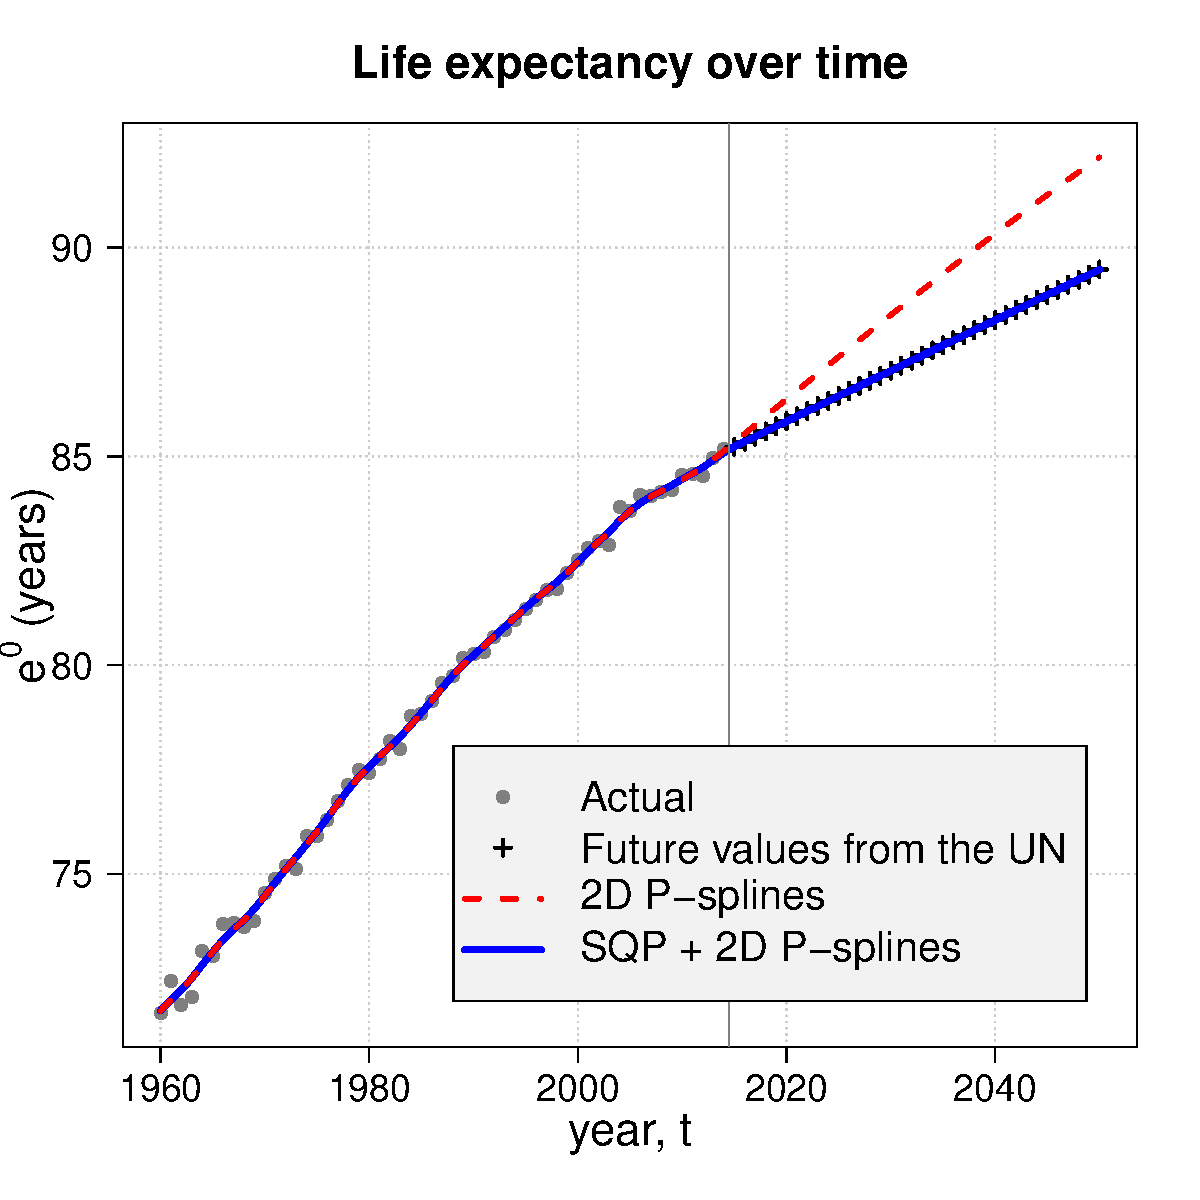
\includegraphics[scale=0.38]{Figures/Camardafig1a.pdf}
	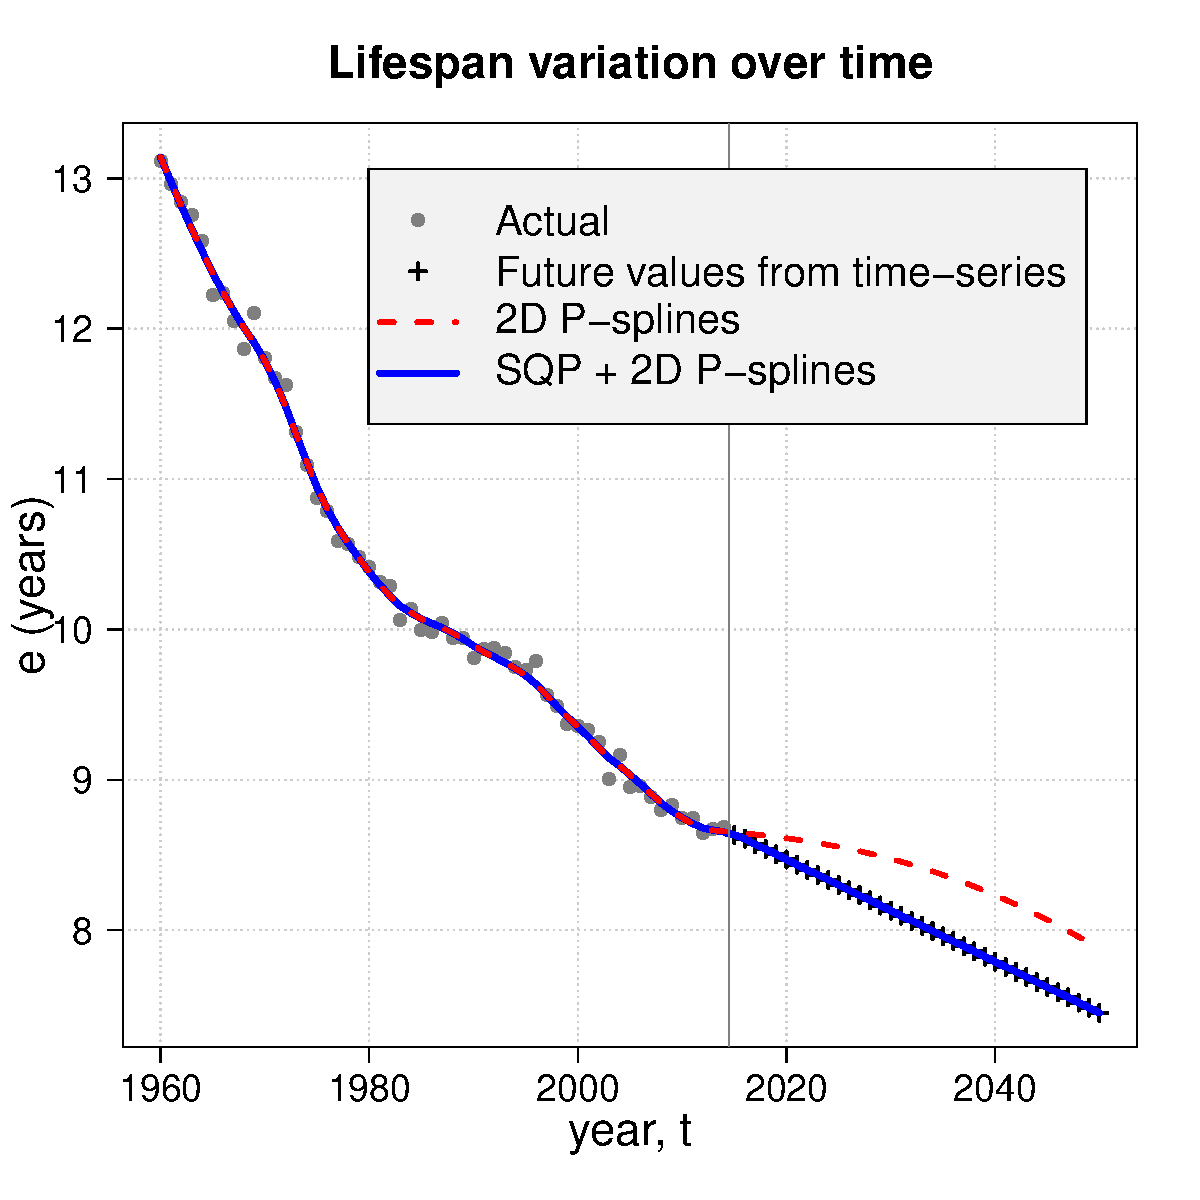
\includegraphics[scale=0.38]{Figures/Camardafig1b.pdf}
	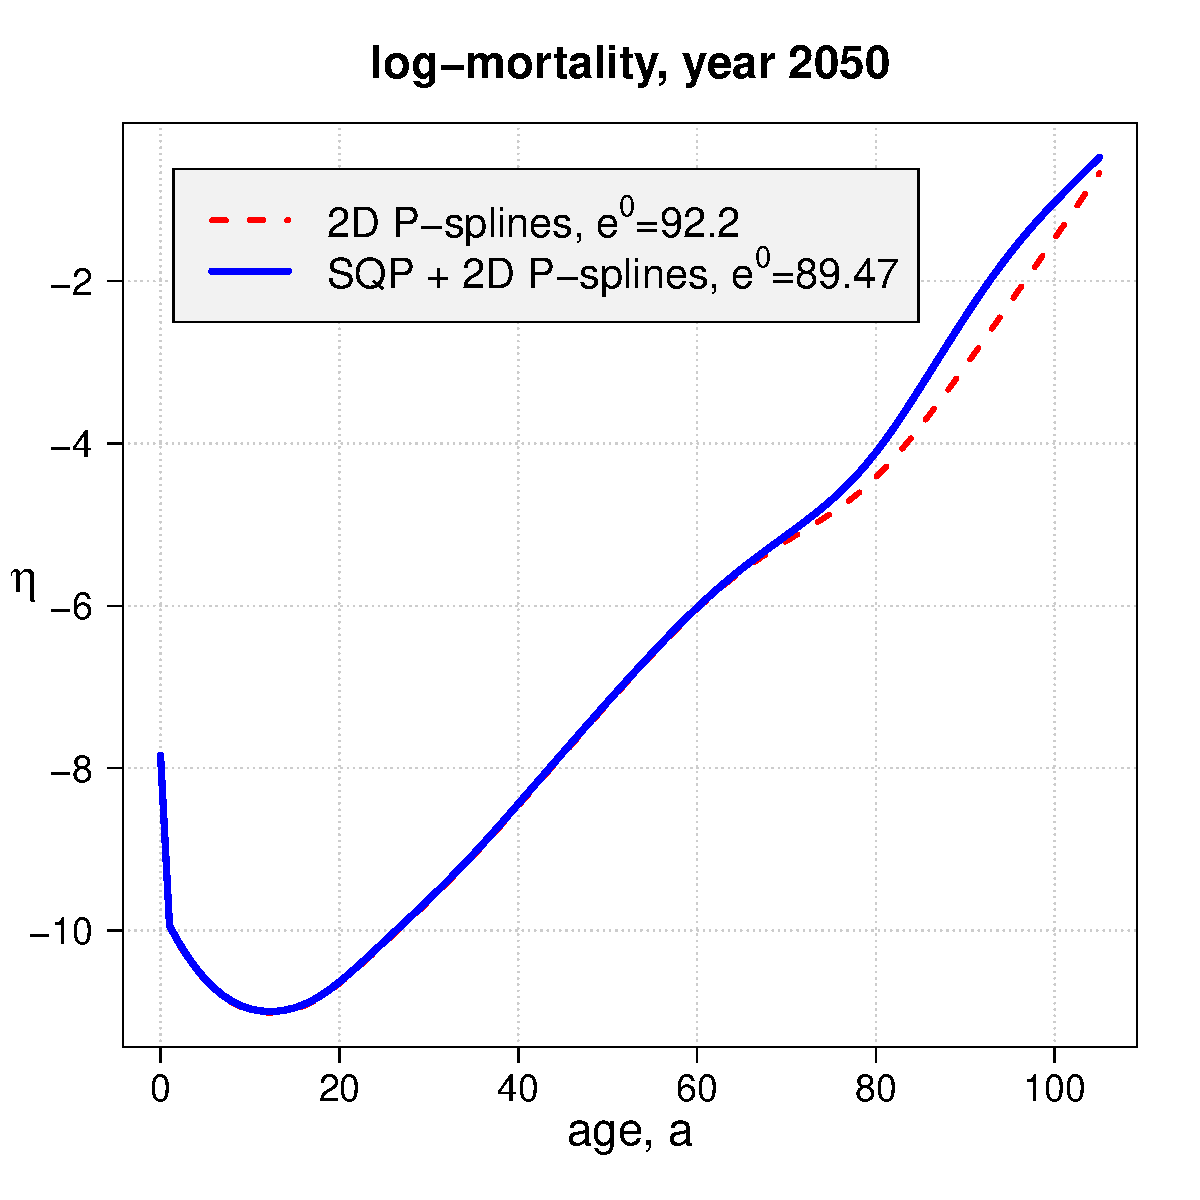
\includegraphics[scale=0.38]{Figures/Camardafig1c.pdf}
	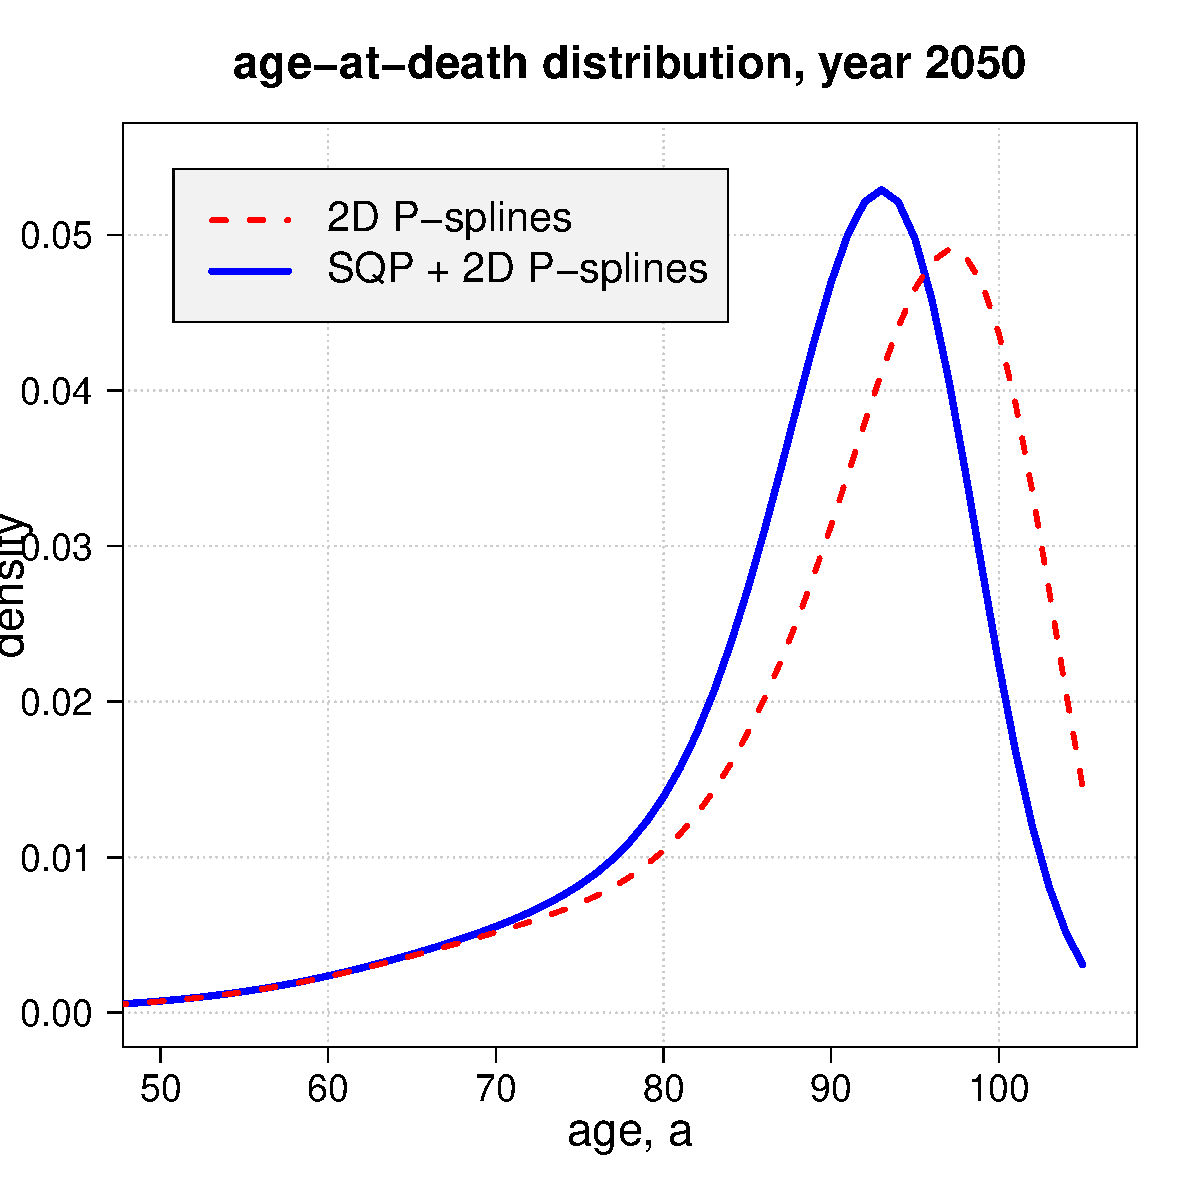
\includegraphics[scale=0.38]{Figures/Camardafig1d.pdf}
	\caption{\label{fig:CamardaMort} Top panels: Actual, estimated and forecast life expectancy at birth and lifespan disparity measure by United Nations and time-series, 2D $P$-splines and the SQP+2D $P$-splines. Bottom panels: Mortality in 2050 described by log-hazards and associated densities (ages 50+) by 2D $P$-splines and the SQP+2D $P$-splines. Italian females, ages 0-105, years 1960-2014, forecast up to 2050.}
\end{figure}


\section{Spanish Fertility Data}

We forecast Spanish fertility using three commonly-used summary measures: Total Fertility Rate describing average number of children per women in a given year, and mean and variance of childbearing age which measure fertility shape over age. In formulas:
\begin{eqnarray}\label{eq:FertMea}
TFR(\bm{\alpha}_{j}) &=& \bm{1}_{m}^{T} \, \bm{\mu}_{j}\\
MAB(\bm{\alpha}_{j}) &=& \bm{\mu}_{j}^{T} \, (\bm{a}+0.5) \; / \; TFR(\bm{\alpha}_{j})\nonumber\\
VAB(\bm{\alpha}_{j}) &=& \bm{\mu}_{j}^{T} \, (\bm{a}+0.5)^2 \; / \; TFR(\bm{\alpha}_{j}) - MAB(\bm{\alpha}_{j})^2\nonumber \, .
\end{eqnarray} 

We forecast trends of these measures by time-series analysis. We then smooth and constrain future fertility age-patterns to comply forecast values of \eqref{eq:FertMea} as in \eqref{eq:SQLalg}. Summary measures as well as fertility rates in 2050 are presented in Figure~\ref{fig:CamardaFert}. Differences between proposed approach and plain 2D $P$-splines are clear. Whereas $P$-splines blindly extrapolate previous trends mainly accounting for the last observed years, the proposed approach enforces future age-patterns to adhere combinations of summary measures, guiding future fertility toward demographic meaningful trends. 

\begin{figure}[!ht]\centering
	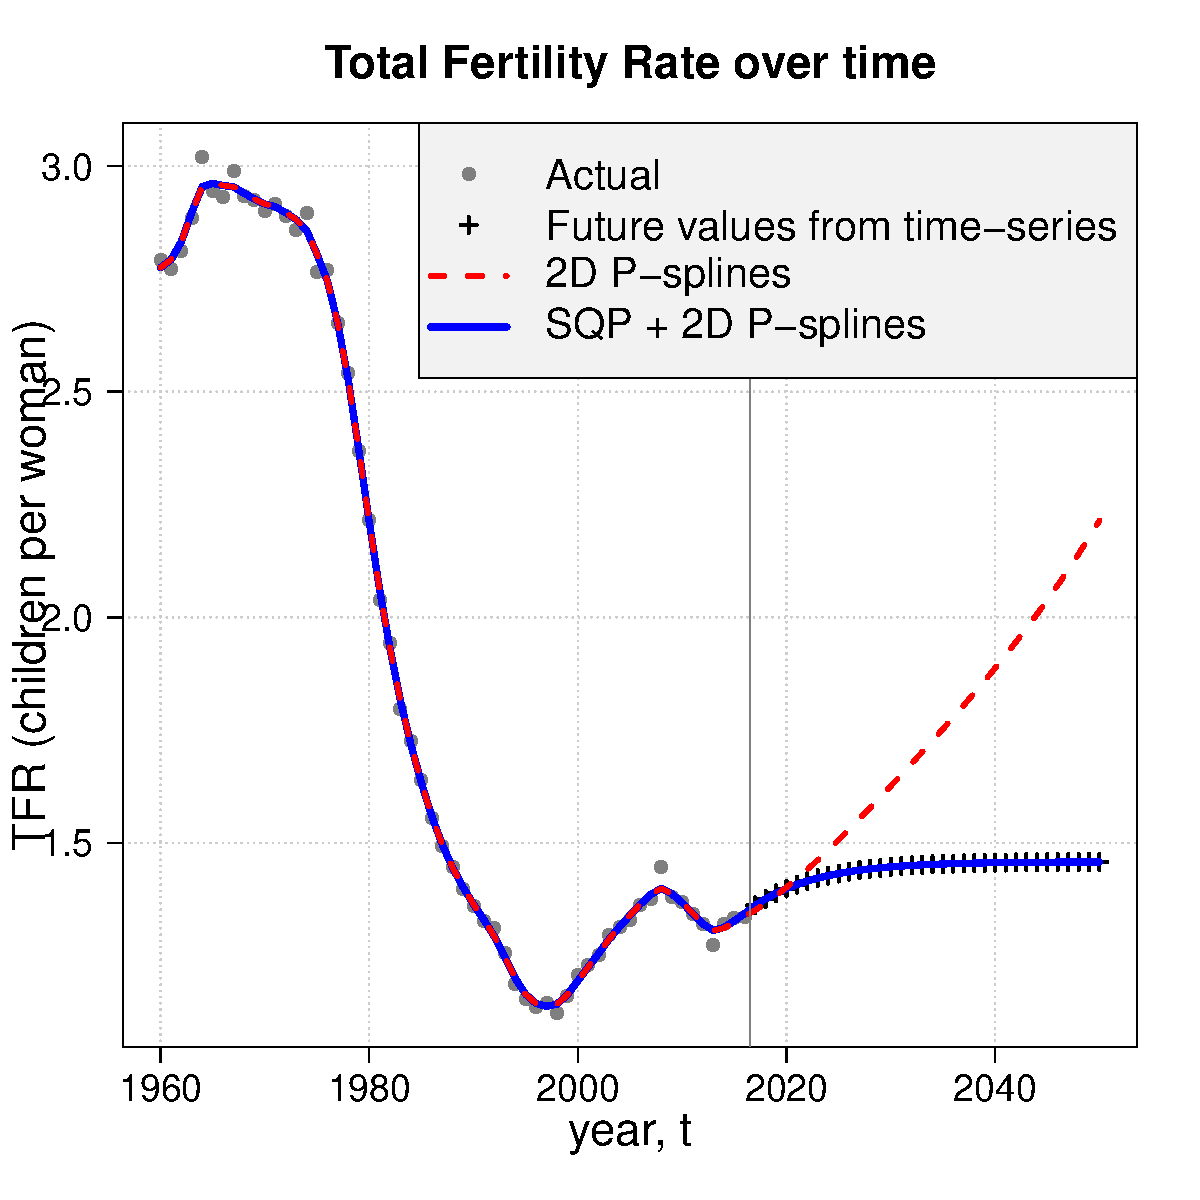
\includegraphics[scale=0.38]{Figures/Camardafig2a.pdf}
	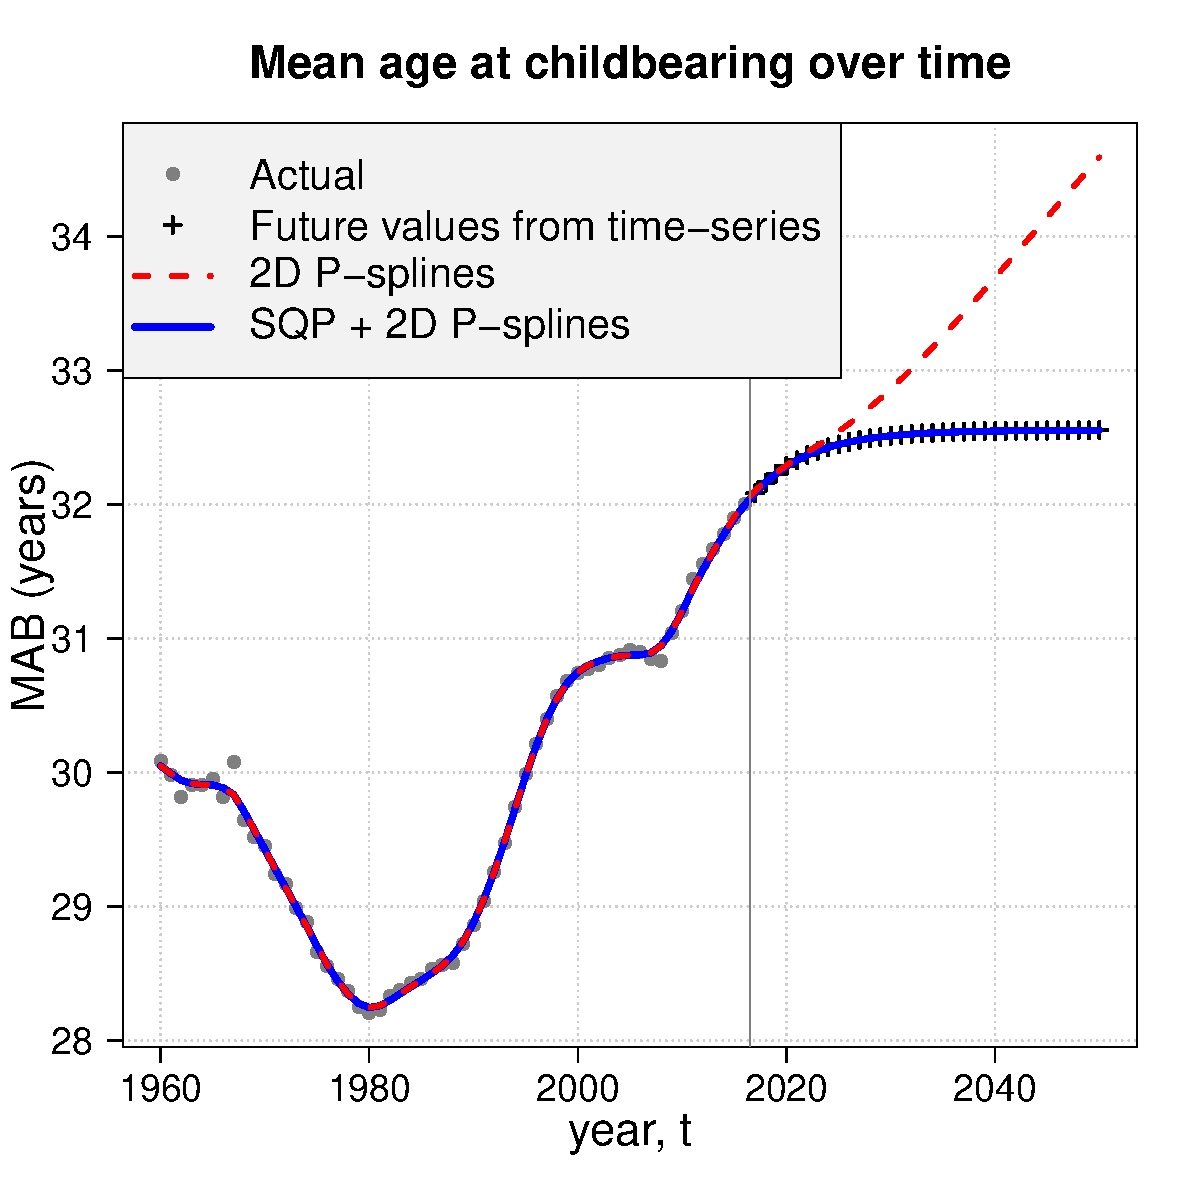
\includegraphics[scale=0.38]{Figures/Camardafig2b.pdf}
	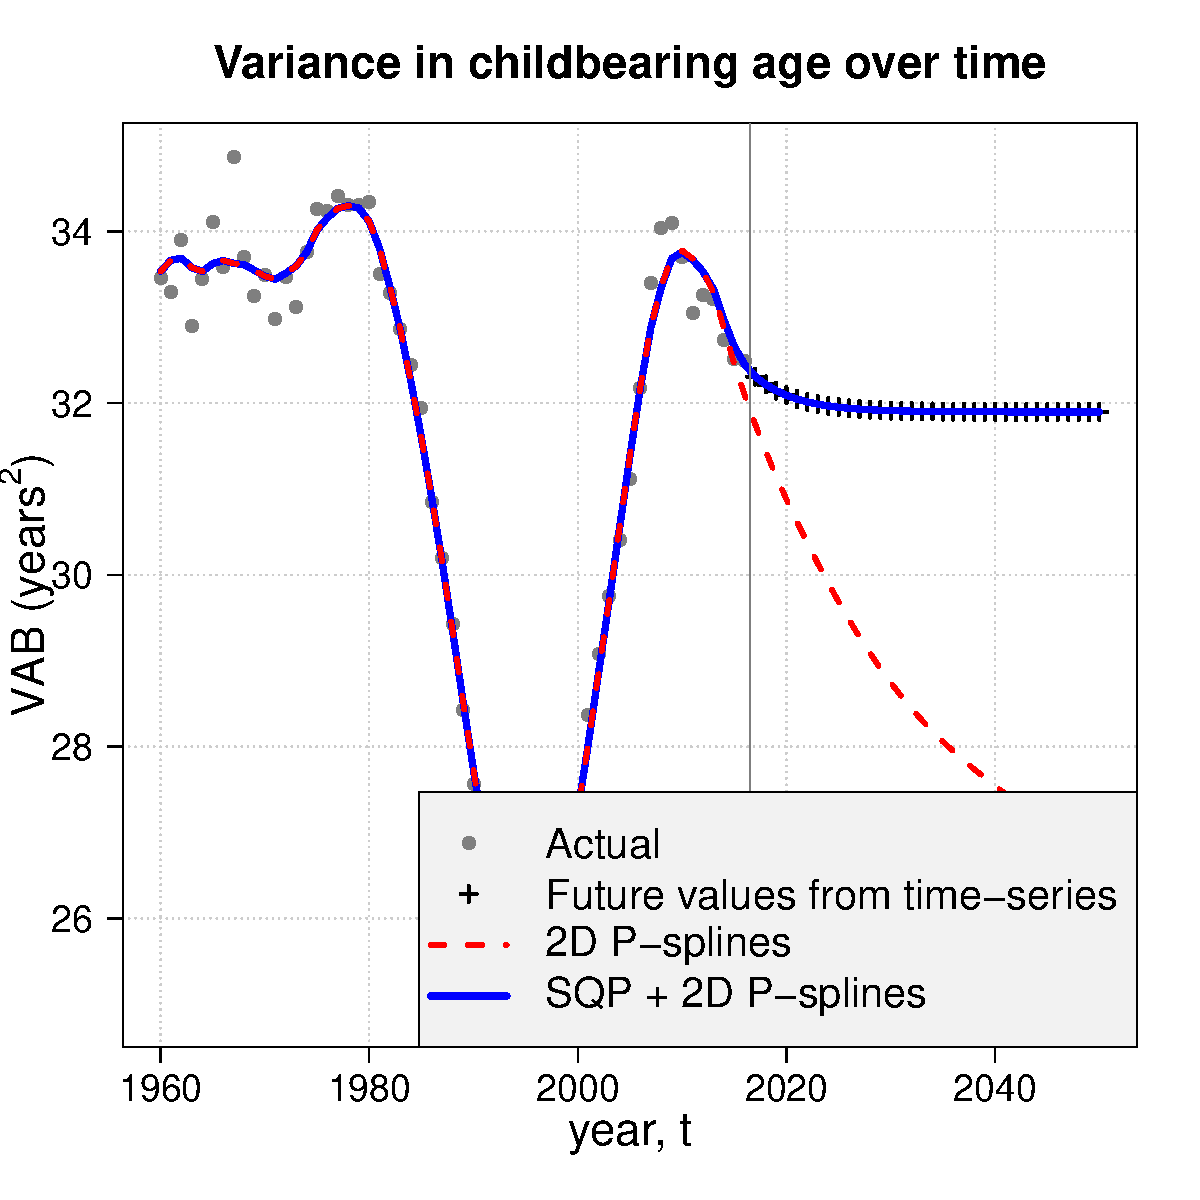
\includegraphics[scale=0.38]{Figures/Camardafig2c.pdf}
	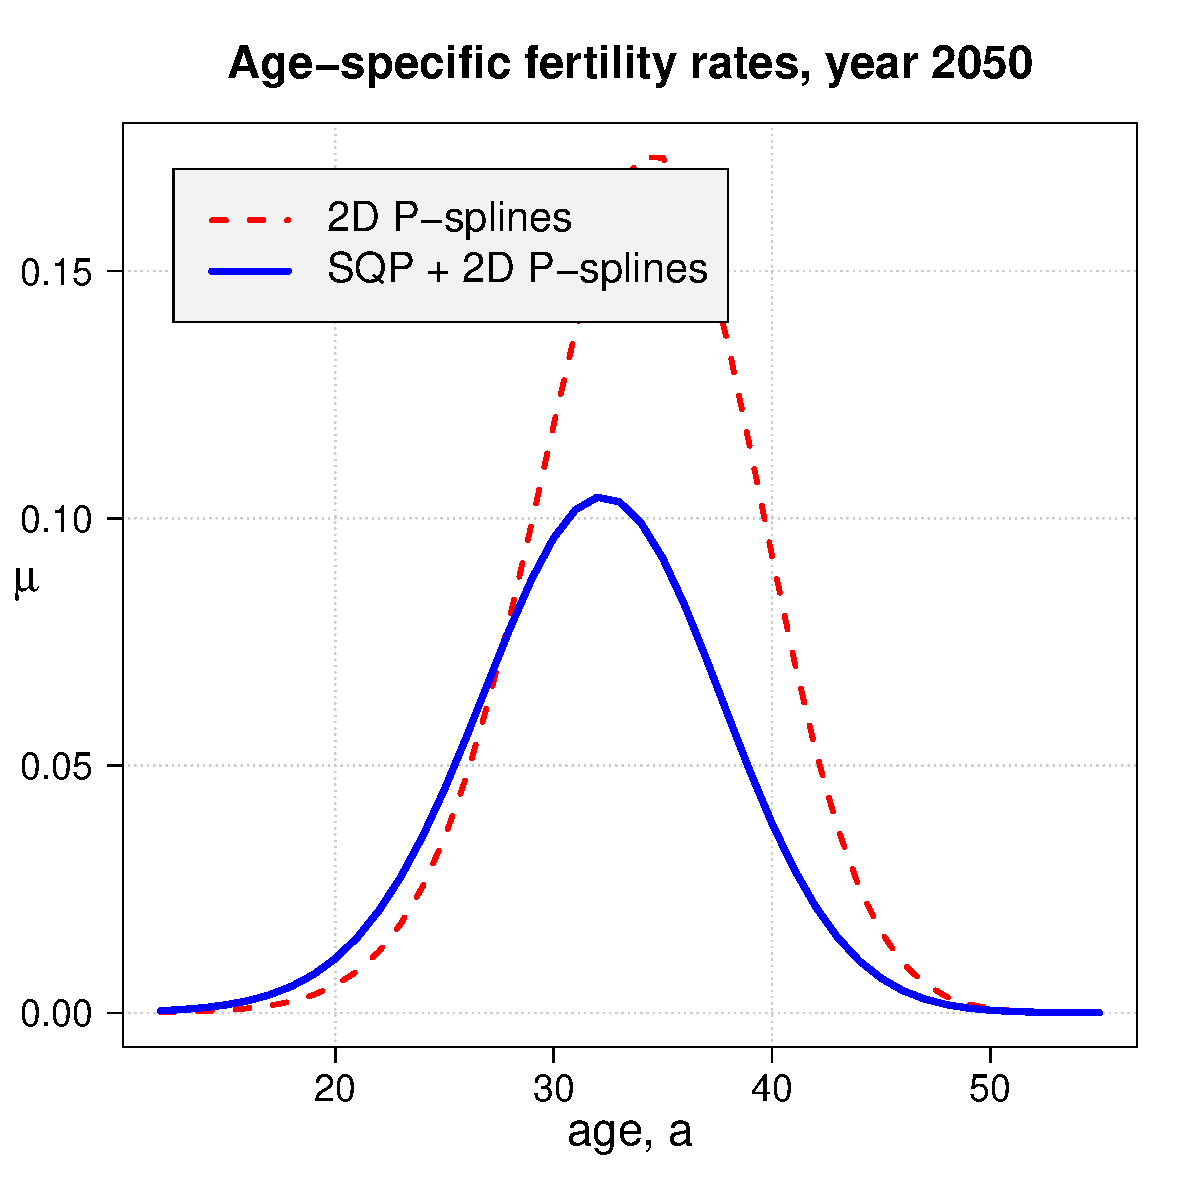
\includegraphics[scale=0.38]{Figures/Camardafig2d.pdf}
	\caption{\label{fig:CamardaFert} Top and left-bottom panels: Actual, estimated and forecast Total Fertility Rate, Mean and Variance in childbearing age by time-series analysis, 2D $P$-splines and the SQP+2D $P$-splines. Right-bottom panel: Age-specific fertility rate in 2050 by 2D $P$-splines and the SQP+2D $P$-splines. Spain, ages 12-55, years 1960-2016, forecast up to 2050.}
\end{figure}

\section{Concluding remarks}

In this paper, we combine smoothing models ($P$-splines) and optimization with nonlinear constraints (Sequential Quadratic Programming) to forecast vital rates when future values of demographic summary measures are provided. 
%The proposed approach allows to obtain smooth future mortality and fertility patterns which comply projected measures commonly easy to interpret and predict. 

We envisage further applications. Forecast of vital rates for partially completed cohorts is often relevant in population studies. For instance, final fertility history of a given cohort may be hypothesized though age-pattern is not yet observed and its estimation will be necessary. We also plan to adopt our approach to reconstruct demographic scenarios which are conventionally based on summary measures. 

From a methodological perspective, future work will be realized to incorporate uncertainty and to objectively select the amount of smoothness in future mortality and fertility age-patterns.

\section{Discussion}



\section*{Appendix A}

The Gini coefficient is an indicator of relative variation. It was originally proposed in Economics to measure income or wealth inequality and  has been adopted in demography and survival analysis to measure lifespan variation \citep{Hanada1983,Shkolnikov2003,bonetti2009gini,gigliarano2017longevity} There exist several alternative and equivalent ways to define the Gini coefficient \citep{yitzhaki2013gini}. For our purposes and the remainder of this article, we will use the following formulation: 
%
\begin{equation}\label{eq:G}
G(\bm{\alpha}_{j}) = \bm{1}_{m}^{T} - \frac{ \bm{1}_{m}^{T} \, \exp[ 2\, \bm{C} \, \bm{\mu}_{j}] }{e^{0} (\bm{\alpha}_{j})}, 
\end{equation}
%
which is equivalent to $G = 1-\frac{\int_0^\infty\ell(x)^2\,dx}{\int_0^\infty\ell(x)\,dx}$ \citep{michettid1957,Hanada1983}.
Where $\int_0^\infty \ell(x)^2\,dx$ is the resulting life expectancy at birth of doubling the hazard at all ages. The Gini coefficient takes values between 0 and 1. A coefficient equal to 0 corresponds to the case of perfect equality in ages at death. The Gini index increases as lifespans become more spread and unequal in the population, reaching a value of 1 in the case of perfect inequality.



% Line interpsace
\linespread{1}\normalsize

% Font size
\small

% References
\bibliographystyle{chicago}
\bibliography{Bib_FertMort}

\end{document} 

